\subsection{Evolução da atitude e modos de operação}
\label{sec:cap4_app_final_atitude}

Ao longo da simulação, a atitude do perseguidor permanece estabilizada em torno da orientação de referência do alvo por conta da lei de controle implementada do tipo \gls{pd}.
As variações mais pronunciadas observadas nos ângulos de Euler $\phi$ (roll), $\theta$ (pitch) e $\psi$ (yaw) concentram-se em transientes rápidos logo após a entrada do controlador de atitude, com duração de fração de segundo, associados à aplicação instantânea do comando de controle.
Esses transientes são interpretados como ruído dinâmico de curta duração e não alteram o resultado final da manobra.
Ao final da aproximação, os erros de atitude convergem para valores próximos de zero, caracterizando um alinhamento consistente do perseguidor em relação ao referencial do alvo e que está dentro do limite máximo estabelecido de $\pm 1^{\circ}$.

\begin{table}[H]
\centering
\caption{Erros de atitude inicial e final do perseguidor em relação ao alvo.}
\label{tab:cap4_app_curta_erros_atitude}
\begin{tabularx}{\linewidth}{|
  >{\centering\arraybackslash}X|
  >{\centering\arraybackslash}X|
  >{\centering\arraybackslash}X|}
\hline
\textbf{Ângulo} &
\textbf{Erro inicial [grau]} &
\textbf{Erro final [grau]} \\
\hhline{|=|=|=|}
$\phi$ (roll)   & $7{,}0^\circ$  & $0{,}51^\circ$ \\
$\theta$ (pitch)& $8{,}0^\circ$  & $0{,}46^\circ$ \\
$\psi$ (yaw)    & $9{,}0^\circ$  & $0{,}50^\circ$ \\
\hline
\end{tabularx}
\end{table}

A Figura~\ref{fig:cap4_app_final_atitude} apresenta a evolução do alinhamento da atitude do perseguidor em relação ao alvo.

\begin{figure}[H]
\centering
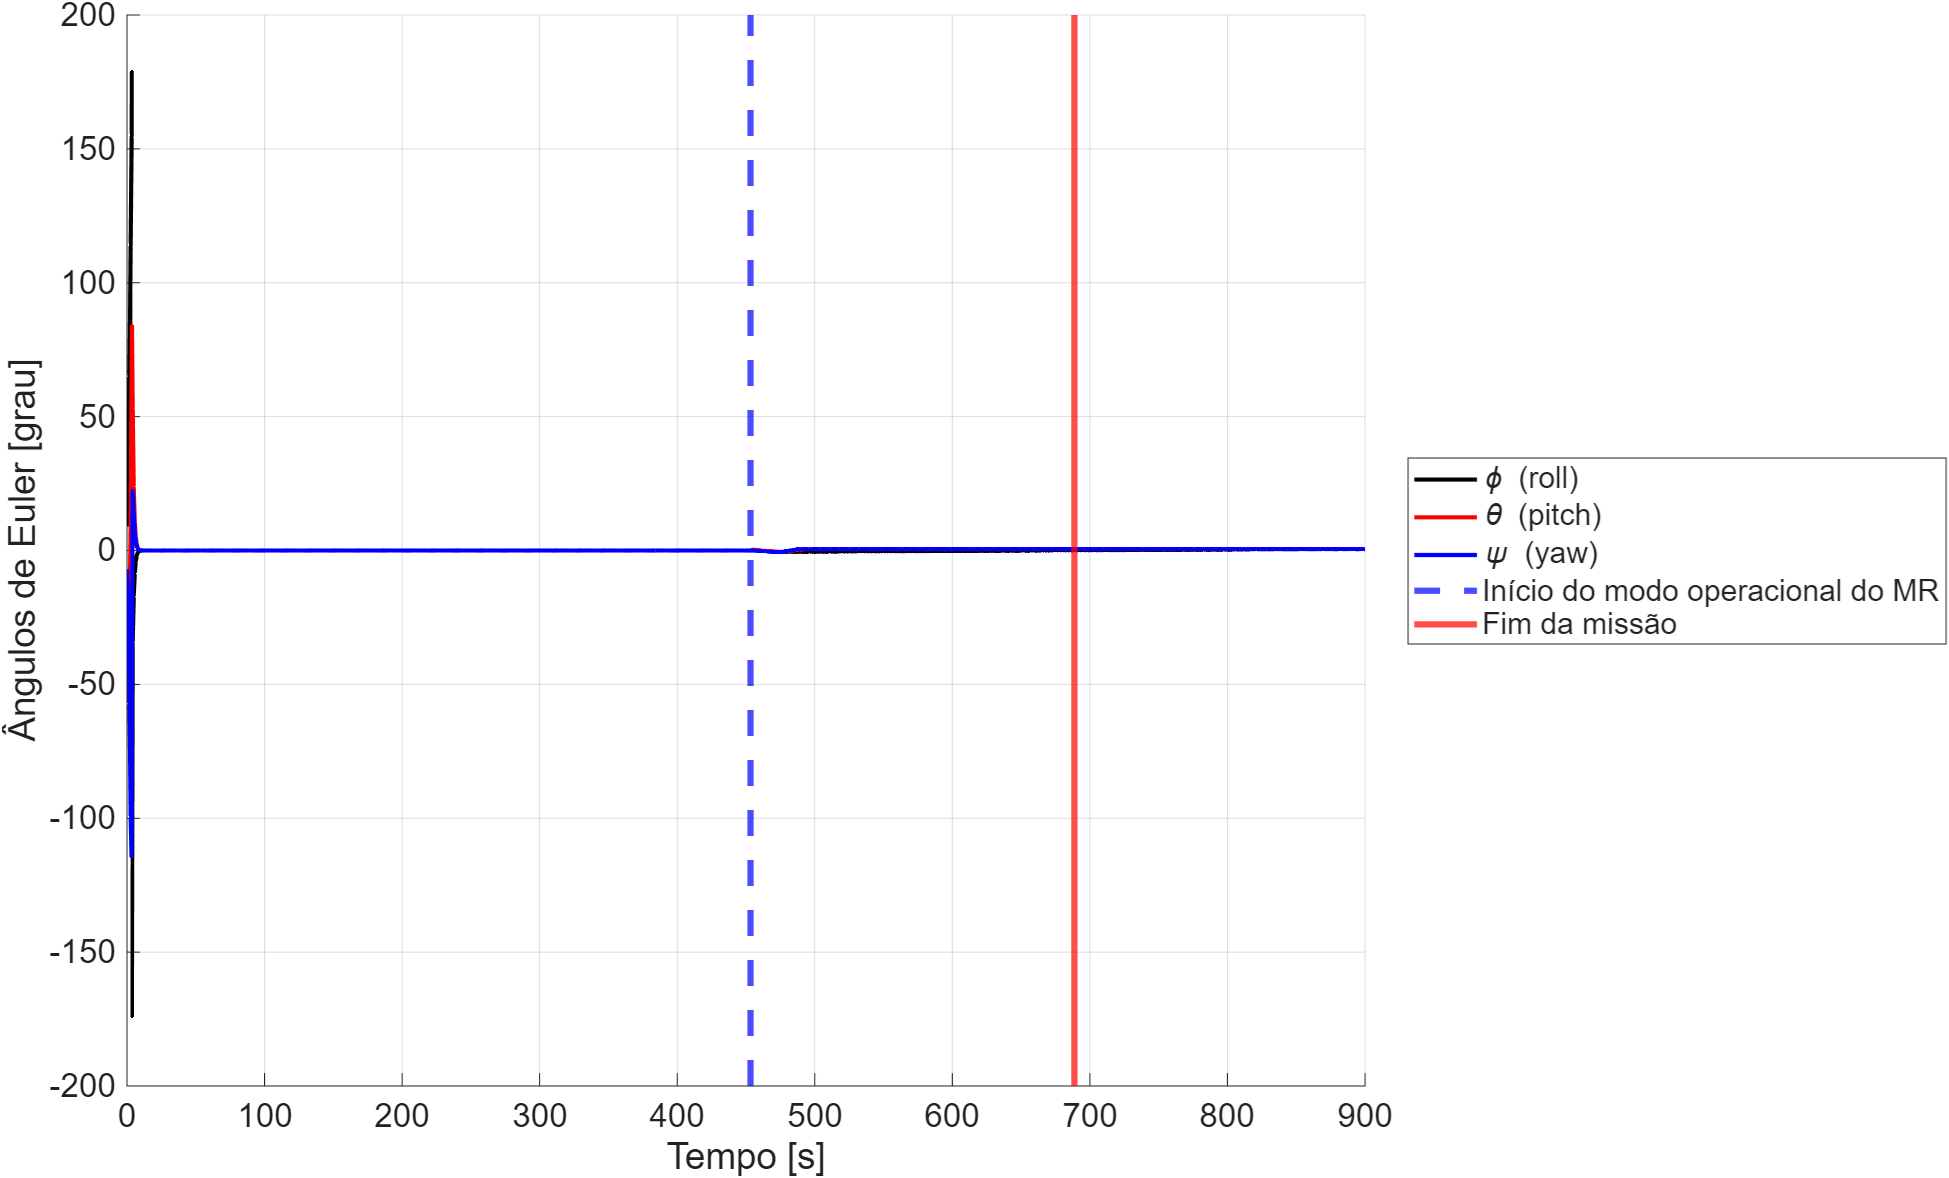
\includegraphics[width=1.0\linewidth]{4 Resultados e discussoes/Imagens/3 App final/1 Atitude perseguidor.png}
\caption{Atitude do perseguidor em ângulos de Euler ao longo de toda a aproximação.}
\label{fig:cap4_app_final_atitude}
\end{figure}

O sinal do modo de operação confirma a lógica de comutação entre a dinâmica de corpo rígido (descrita pelas equações de Euler) e a dinâmica acoplada base--manipulador (equacionamento de Lagrange).
O modo de operação dentro da simulação foi assumido inicialmente o valor $0$, refletindo a fase em que o manipulador não está em operação, e passa para $1$ no instante de habilitação do \gls{mr}, permanecendo igual a $1$ até o final da simulação. Dessa forma, a aproximação final ocorre integralmente sob o modo operacional com o manipulador ativo, combinando controle de atitude do corpo com o movimento coordenado das juntas.

\begin{figure}[H]
\centering
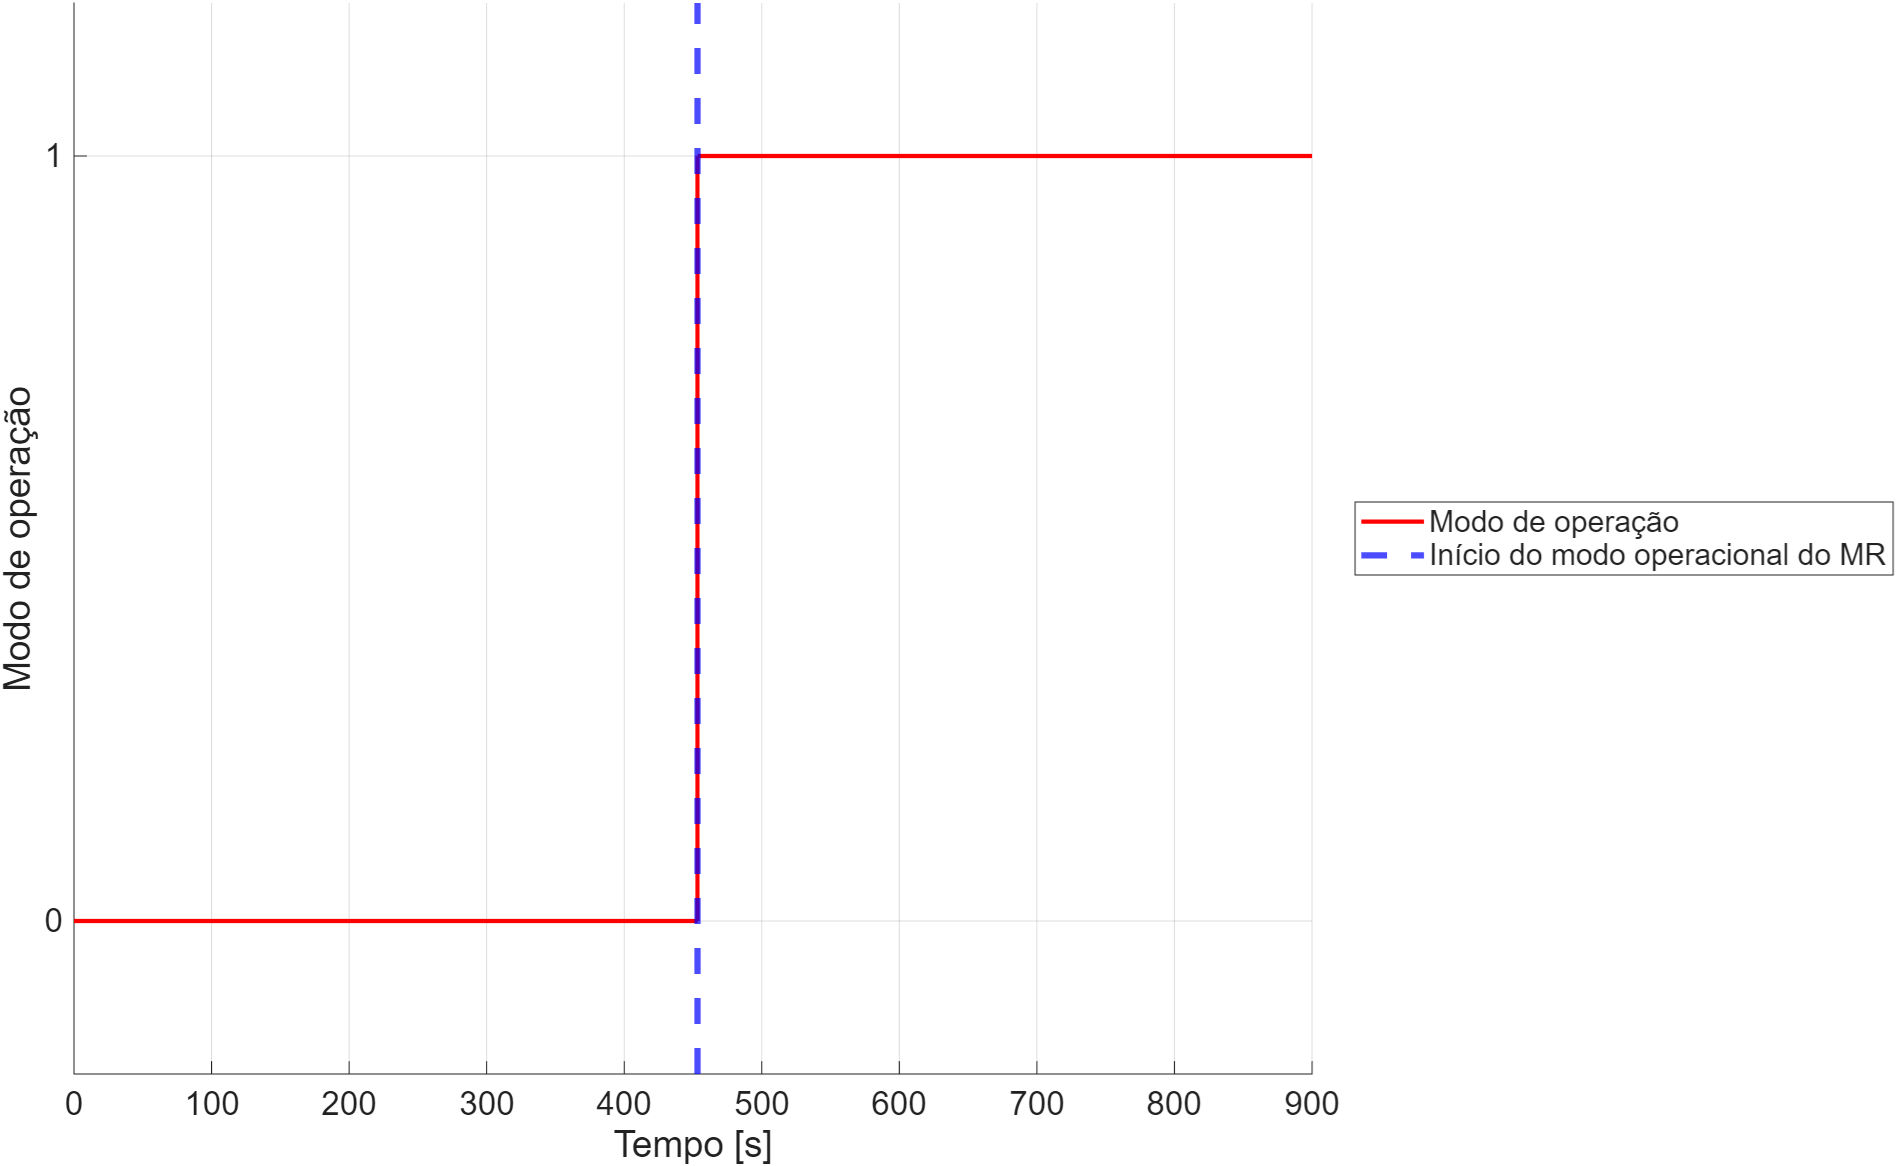
\includegraphics[width=1.0\linewidth]{4 Resultados e discussoes/Imagens/3 App final/1 Modo operacao.png}
\caption{Evolução do modo de operação da dinâmica (modelo de Euler e modelo de Lagrange)}
\label{fig:cap4_app_final_modo_operacao}
\end{figure}

De forma paralela à evolução da aproximação final, o movimento relativo orbital entre perseguidor e alvo continua ativo e ainda sendo descrito pelas equações de \gls{hcw} juntamente com a sua própria lei de controle.